\section{Erster Lösungsansatz
\label{perturbation:section:ersterloesungsansatz}}
\rhead{Erster Lösungsansatz}

Die Formeln \eqref{eq:x_simple} sind ohne viel Rechenleistung berechenbar und somit auch als Flugobjekt durchführbar.
Die Störungstheorie befasst sich damit, die Anfangswerte $x_0$, $y_0$, $v_{0x}$ und $v_{0y}$ so abzuändern,
dass dennoch gute Approximationen für $x(t)$ und $y(t)$ gefunden werden können.
Hierbei ist es die Aufgabe der Bodenstation, die notwendigen Startparameter dem Flugobjekt mitzuteilen,
sodass dieses die Berechnung auf Basis der trivialen Formeln \ref{eq:x_simple}  vornehmen kann.

Als ersten Lösungsansatz haben wir $v_{0x}$ und $v_{0y}$ durch lineare Funktionen abhängig von der Zeit ersetzt, aber $x_0$ und $y_0$ vorerst unberührt gelassen.
Hintergrund dieser Überlegung ist, dass der Luftwiderstand nur die Geschwindigkeit beeinflusst.
\begin{equation*}
	\begin{aligned}
		v_{0x} \rightarrow v_{0x}(t) = v_{0x} + \phi_x \cdot t\\
		v_{0y} \rightarrow v_{0y}(t) = v_{0y} + \phi_y \cdot t
	\end{aligned}
\end{equation*}



Wir passen die Startgeschwindigkeit im Verlaufe der Zeit $t$ also anhand eines unbekannten Faktors $\phi$ an.
Eingesetzt in die Formeln \eqref{eq:x_simple} erhalten wir:
\begin{equation}\label{eq:x_linear}
\begin{aligned}
    x(t) &= x_0 + t \cdot (v_{0x} + \phi_x \cdot t) \\
    y(t) &= y_0 + t \cdot (v_{0y} + \phi_y \cdot t) - \frac{1}{2}gt^2
\end{aligned}
\end{equation}

$x_0$, $y_0$, $v_{0x}$ und $v_{0y}$ sind die bekannten Anfangsbedingungen des Problems.
Ebenfalls können $x(t)$ und $y(t)$ mit dem Runge-Kutta-Verfahren bestimmt werden.
Um neue Werte mit der Störung zu bestimmen, müssen die Unbekannten $\phi_x$ und $\phi_y$ berechnet werden.
Dies kann erreicht werden, indem man die Gleichungen \eqref{eq:x_linear} nach $\phi_x$ bzw. $\phi_y$ auflöst:
\begin{equation}
	\begin{aligned}
	\phi_x &= \frac{x(t) - x_0 - tv_{0x}}{t^2}\\
	\phi_y &= \frac{y(t) - y_0 - tv_{0y} + \frac{1}{2}gt^2}{t^2}
	\end{aligned}
\end{equation}

Beispielsweise kann dieses Gleichungssystem für $t = 5s$ gelöst werden.
Dadurch erhält man $\phi_x$ und $\phi_y$.
Da hierzu allerdings $x(t=5)$ und $y(t=5)$ mittels Runge-Kutta berechnet werden müssen, ist dazu nur die Bodenstation in der Lage.
Die Werte $\phi_x$ und $\phi_y$ können nun aber dem Flugobjekt übertragen werden,
welches mit den Formeln \eqref{eq:x_linear} seine Position in naher Zukunft nun autonom approximieren kann,
beispielsweise für das Intervall $t \in [5,6)$.
Anschliessend könnte die Bodenstation die Werte $\phi_x$ und $\phi_y$ für $t=6s$ neu berechnen, um den Fehler nicht beliebig anwachsen zu lassen.

Das Resultat ist in Abbildung \ref{naive_linear_term} dargestellt.
Grün ist dabei die exakte Flugbahn gemäss den Differentialgleichungen \eqref{eq:x_diff},
blau die linear berechnete Bahn ohne Berücksichtigung des Luftwiderstandes und
rot die korrigierte Variante.
Für die korrigierte Variante wurde eine Intervalllänge von $t=1s$ gewählt.
Das heisst, sie bestimmt die Unbekannten $\phi_x$ und $\phi_y$ zu jeder vollen Sekunde $t \in \{1, 2, 3, \cdots, 25\}$ und nutzt jene Daten,
um die Position jeweils für die folgende Sekunde vorherzusagen.
Wie zu erkennen ist, kann ein Grossteil des Fehlers bereits vermieden werden.
\begin{figure}
    \centering
    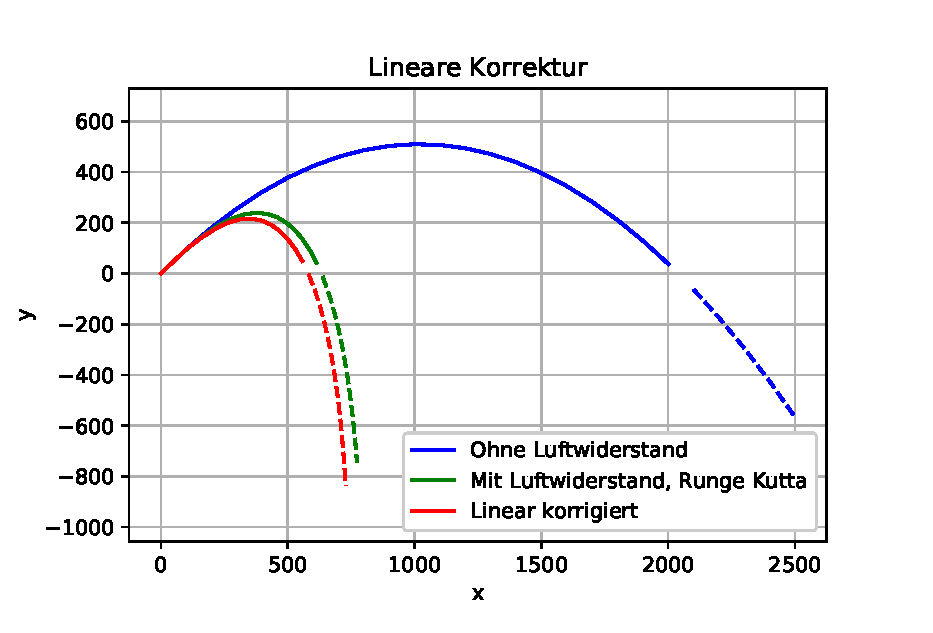
\includegraphics[scale=0.7]{papers/perturbation/bilder/perturbation_fig1.eps}
    \caption{Linearer Korrekturterm}
	\label{naive_linear_term}
\end{figure}


Anstelle des linearen Ansatzes könnte man auch einen quadratischen Ansatz nutzen.
Dies ergibt anstelle von \eqref{eq:x_linear}:
\begin{equation}
\begin{aligned}
x(t) &= x_0 + t \cdot (v_{0_x} + \phi_{x_1}t + \phi_{x_2}t^2) = x_0 + v_{0_x}t + \phi_{x_1}t^2 + \phi_{x_2}t^3\\
y(t) &= y_0 + t \cdot (v_{0_y} + \phi_{y_1}t + \phi_{y_2}t^2) - \frac{1}{2}gt^2 = y_0 + v_{0_y}t + \phi_{y_1}t^2 + \phi_{y_2}t^3 - \frac{1}{2}gt^2
\end{aligned}
\end{equation}


Damit haben wir noch bessere Resultate erhalten.
Diese sind in Abbildung \ref{naive_quadratic_term} ersichtlich.
Von Auge ist bereits kein Unterschied der beiden Flugbahnen mehr erkennbar.
\begin{figure}
    \centering
    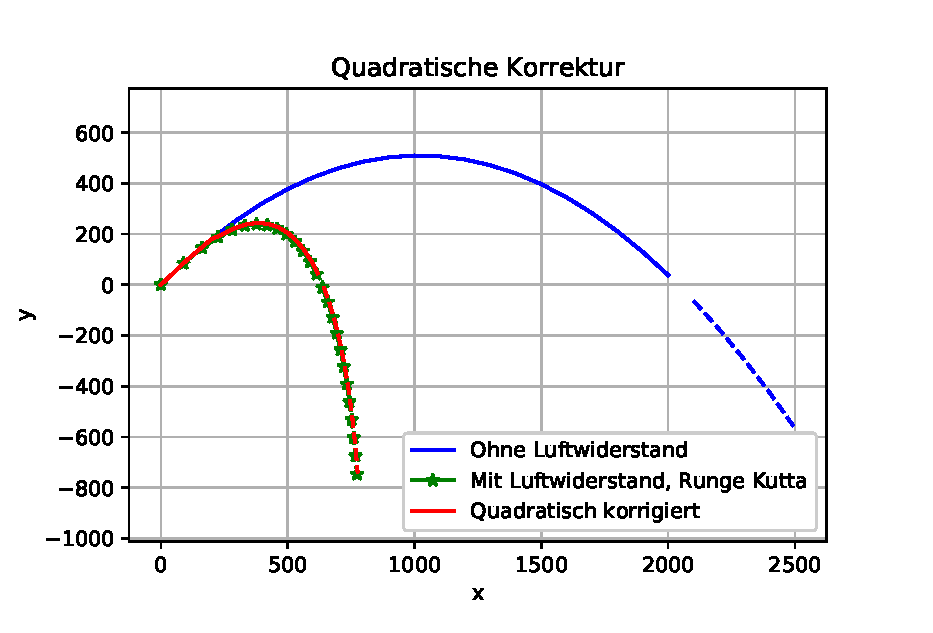
\includegraphics[scale = 0.7]{papers/perturbation/bilder/perturbation_fig2.eps}
    \caption{Quadratischer Korrekturterm}
	\label{naive_quadratic_term}
\end{figure}